\documentclass{beamer}
\usepackage[utf8]{inputenc}    
\setbeamertemplate{navigation symbols}{}
\beamertemplatenavigationsymbolsempty{}
\setbeamertemplate{footline}[frame number]
\usepackage[T1]{fontenc}
\usepackage{babel}
\usepackage{subcaption}
\usepackage{caption}
\usepackage{graphicx}
\usepackage{lmodern}
\setbeamercovered{transparent}
\setbeamertemplate{page number in head/foot}[totalframenumber]
\usetheme{Copenhagen}       
\title{Machine Learning I} 
\author[Ricardo Figueiredo, Sérgio Cardoso]{
    Ricardo Figueiredo up202105430 
    \and  \\
    Sérgio Cardoso up202107918
}

\begin{document}
\maketitle

\begin{frame}{Executive Summary}
    \begin{itemize}
        \item \textbf{Goals:} use a classification algorithm taught on classes 
        to evaluate its performance on a set of benchmark datasets.
        \pause
        \item \textbf{Outline of the Approach:} base our implementation on 
        open-source code, then modify it 
        in order to make it more robust to the data 
        characteristic in question.
        \pause
        \item \textbf{Summary of Results:} 
        \begin{itemize}
            \item Tables comparing Accuracy/F1-Score/Precision/Recall/ROC across datasets
            \item Comparison of the original and modified algorithms
            \item Summary of the improvement of the algorithm
            (modified vs original)
        \end{itemize}
    \end{itemize}
\end{frame}

\begin{frame}{Selected Algorithm} 
    For this assignment, we chose the CART algorithm due to its easy learning curve. 
    CART stands for Classification And Regression Tree which, in 
    itself, uses a Decision Tree. 
    Decision Trees are among the most popular models in ML, as they are used 
    not only by CART, but also by other algorithms, such as ID3 (Iteractive 
    Dichotomiser 3) or C4.5, the latter being an extension of CART. \\  
    CART uses the Gini index as its impurity measure: given a data set D = $\{ \langle x_{i}, 
        y_{i}\rangle \}_{i = 1}^{N}$ (with N examples), $Gini(D) = 1 - \sum_{i = 1}^{c} {p_{i}}^2$, where
        $p_{i}$ is the probability of class i. \\
\end{frame}

\begin{frame}{Data Characteristic}
    Decision trees, when working with imbalanced datasets, 
    emphasize the majority class (the one with more examples), 
    which can lead to high misclassification rates for the 
    minority classes. \\
    There are some ways to prevent this from happening, such as:
    \begin{itemize}
        \item Cost-Sensitive Learning (assign higher misclassification costs 
        to the minority class)
        \item Sampling Techniques (balance the dataset by oversampling 
        the minority class (using SMOTE) or undersampling 
        the majority class (Tomek Links, ENN - Edited Nearest
        Neighbors))
        \item Alternative Evaluation Metrics to Accuracy (e.g. Precision, Recall or
        F1-Score)
    \end{itemize}
\end{frame}

\begin{frame}{Proposal}
We were given the three following sets 
    of benchmark datasets:
    \begin{enumerate}
       \item Noise or Outliers 
       \item Class Imbalance in Binary Classification
       \item Multiclass Classification 
    \end{enumerate}
    Since CART uses Binary Partitioning, we ended up using the 
    set of binary classification datasets 
    (Class Imbalance in Binary Classification). We also used this 
    set because of the fact that CART can deal with class 
    imbalanced data, if we apply some of the techniques mentioned 
    before. 
\end{frame}      

\begin{frame}{Empirical Study}
    \textbf{Experimental Setup:} 
    \begin{itemize} 
        \item Datasets: unbalanced binary classification datasets. 
        \item Hyperparameters of the Algorithm:
        \begin{itemize}
            \item Maximum Depth of the Tree 
            \item Criterion (Gini)
            \item Class Weight 
        \end{itemize}
    \end{itemize} 
    \pause
    \textbf{Performance Estimation Methodology:} \\ Since most 
    of the datasets tested for this assignment are so large, we used
    the holdout method, in which we split the data in two 
    sub-sets: one for training and the other for testing.
\end{frame}

\begin{frame}{Empirical Study - Performance of the original CART algorithm}
    \begin{figure}
            \centerline{%
            \subfloat[Accuracy]{
                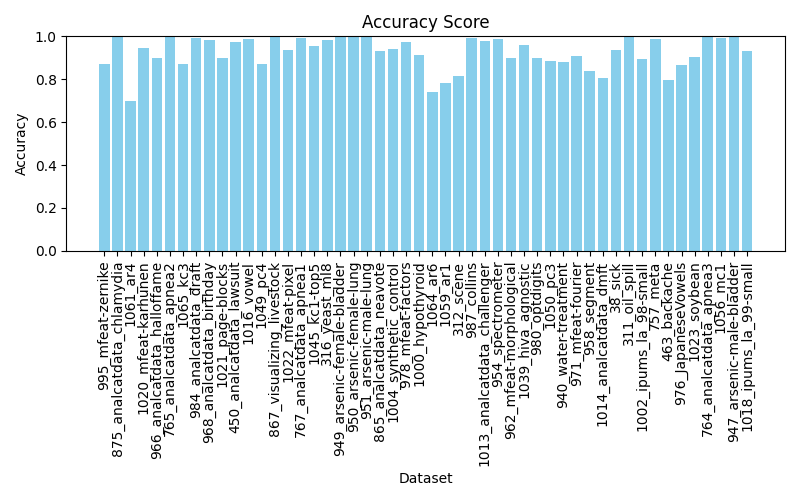
\includegraphics[width=.47\textwidth]{results/accuracy_plot.png}
            }\hfill
            \subfloat[Precision]{
                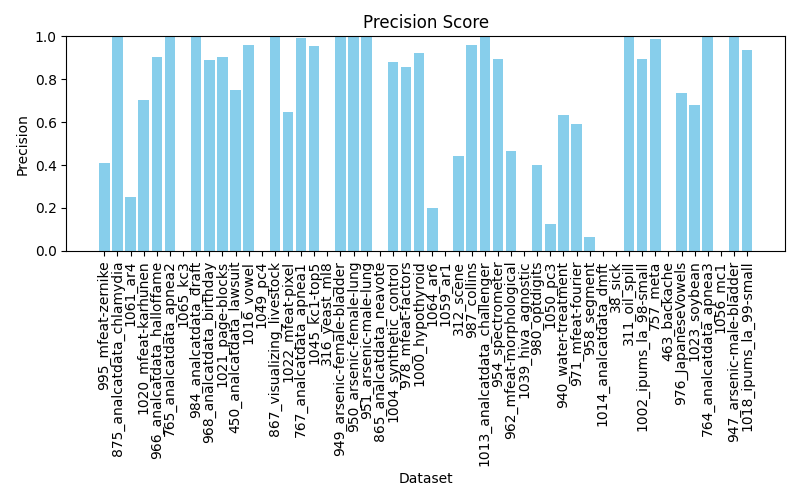
\includegraphics[width=.47\textwidth]{results/precision_plot.png}
            }%
            }
            \centerline{%
            \subfloat[Recall]{
                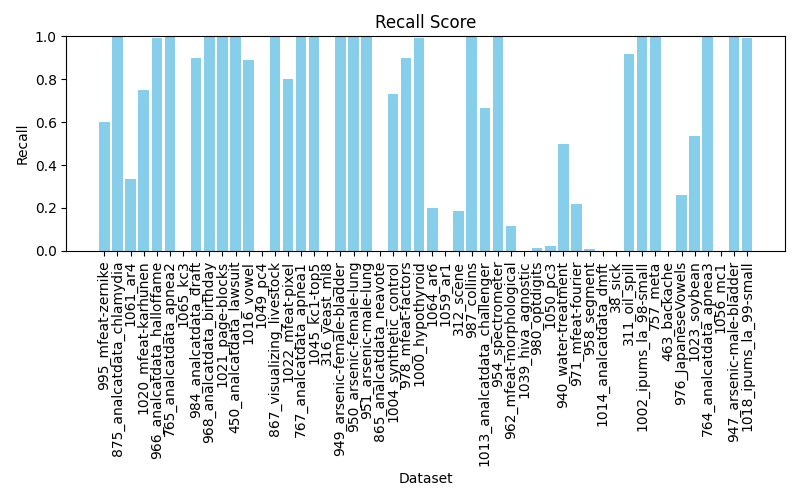
\includegraphics[width=.37\textwidth]{results/recall_plot.png}
            }\hfill
            \subfloat[F1-Score]{
                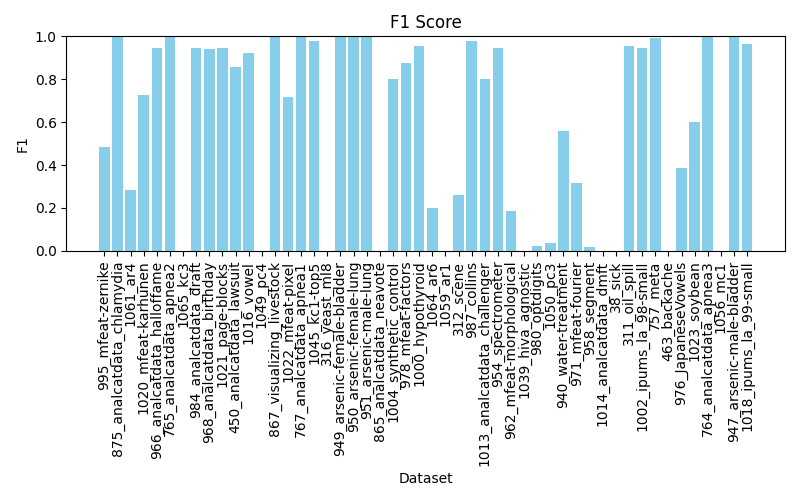
\includegraphics[width=.37\textwidth]{results/f1_plot.png}
            }\hfill
            \subfloat[ROC]{
                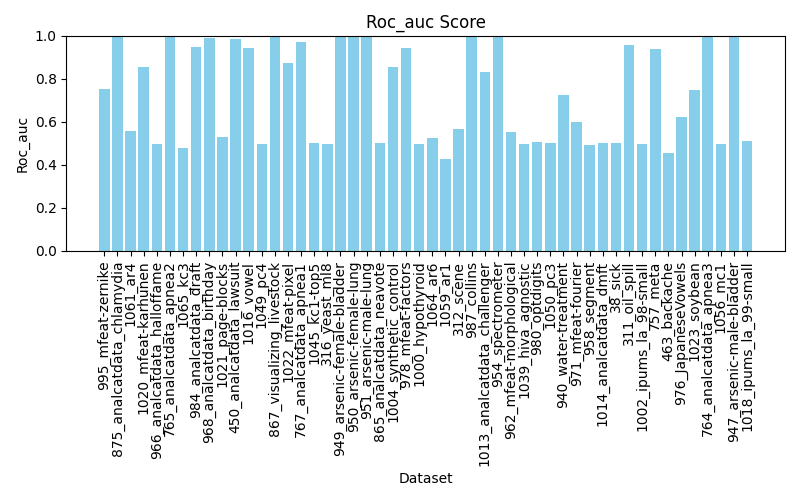
\includegraphics[width=.37\textwidth]{results/roc_auc_plot.png}
            }%
            }
    \end{figure}
\end{frame}

\begin{frame}{Empirical Study - Performance of the modified CART algorithm}
    \begin{figure}
            \centerline{%
            \subfloat[Accuracy]{
                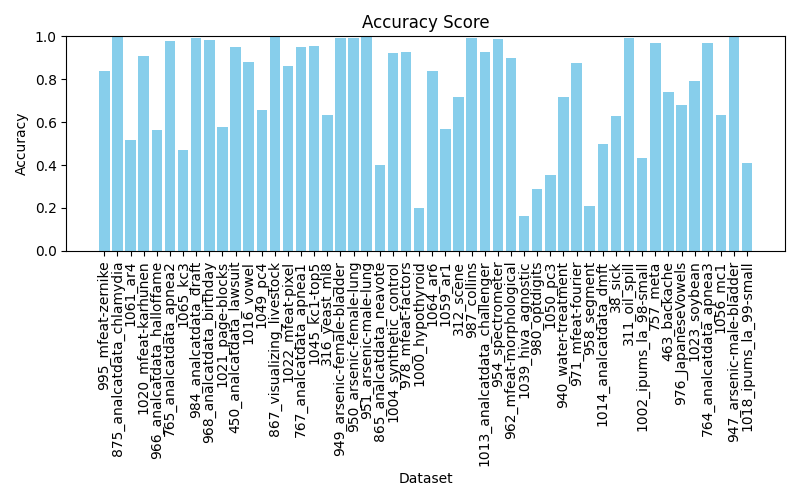
\includegraphics[width=.47\textwidth]{results/newaccuracy_plot.png}
            }\hfill
            \subfloat[Precision]{
                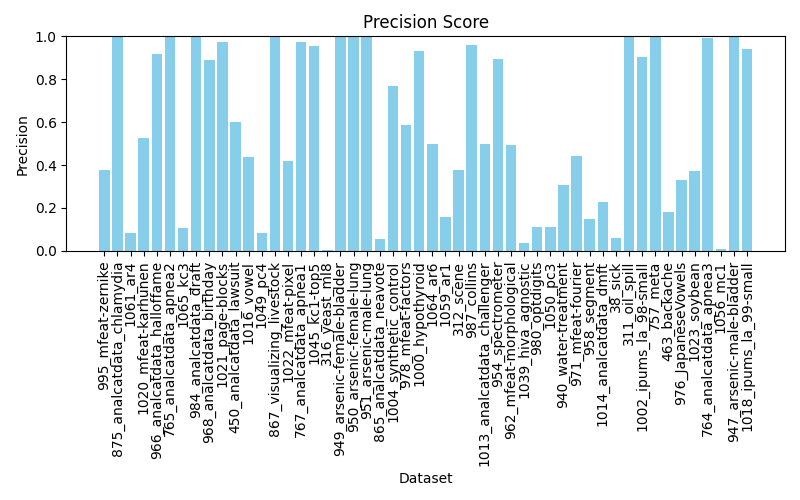
\includegraphics[width=.47\textwidth]{results/newprecision_plot.png}
            }%
            }
            \centerline{%
            \subfloat[Recall]{
                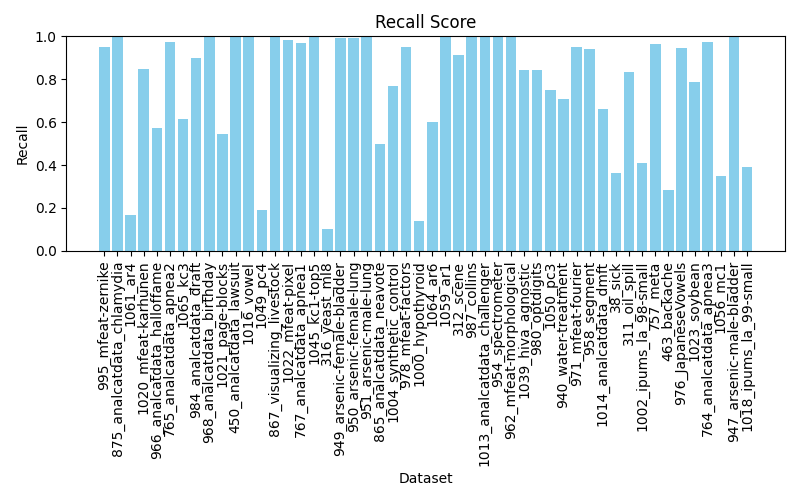
\includegraphics[width=.37\textwidth]{results/newrecall_plot.png}
            }\hfill
            \subfloat[F1-Score]{
                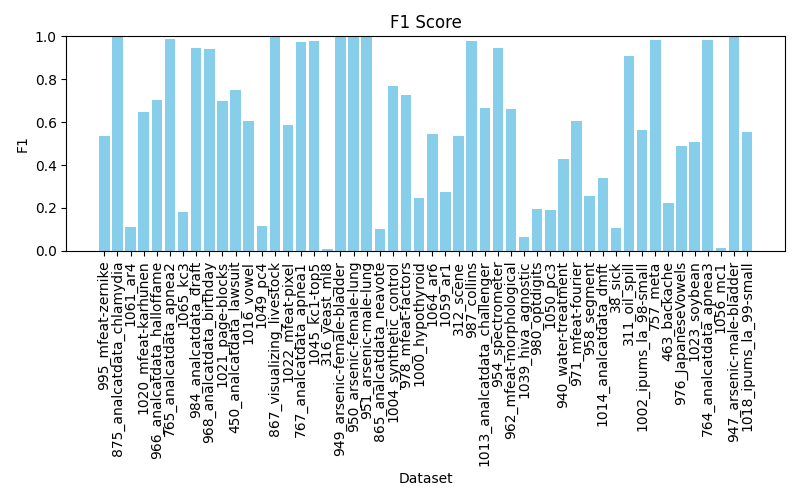
\includegraphics[width=.37\textwidth]{results/newf1_plot.png}
            }\hfill
            \subfloat[ROC]{
                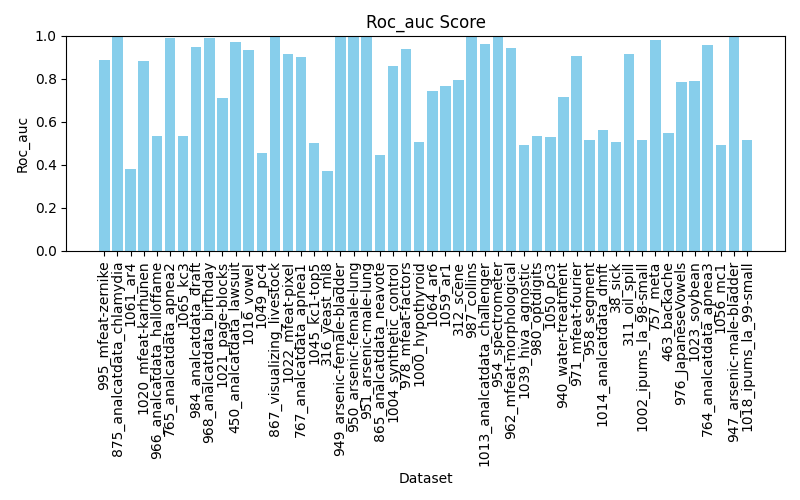
\includegraphics[width=.37\textwidth]{results/newroc_auc_plot.png}
            }%
            }
    \end{figure}
\end{frame}

\begin{frame}{Empirical Study - Performance Comparison}
    \begin{figure}
            \centerline{%
            \subfloat[Accuracy]{
                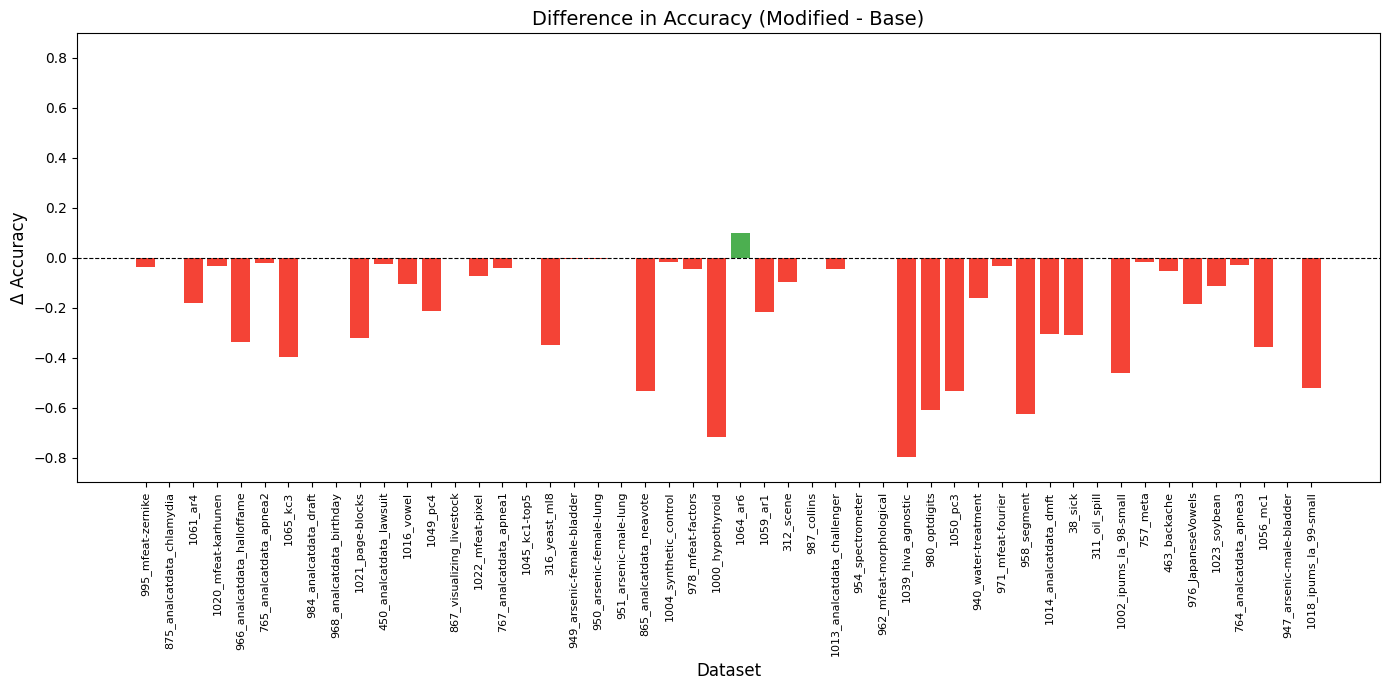
\includegraphics[width=.47\textwidth]{results/comparisons/accuracy_comparison.png}
            }\hfill
            \subfloat[Precision]{
                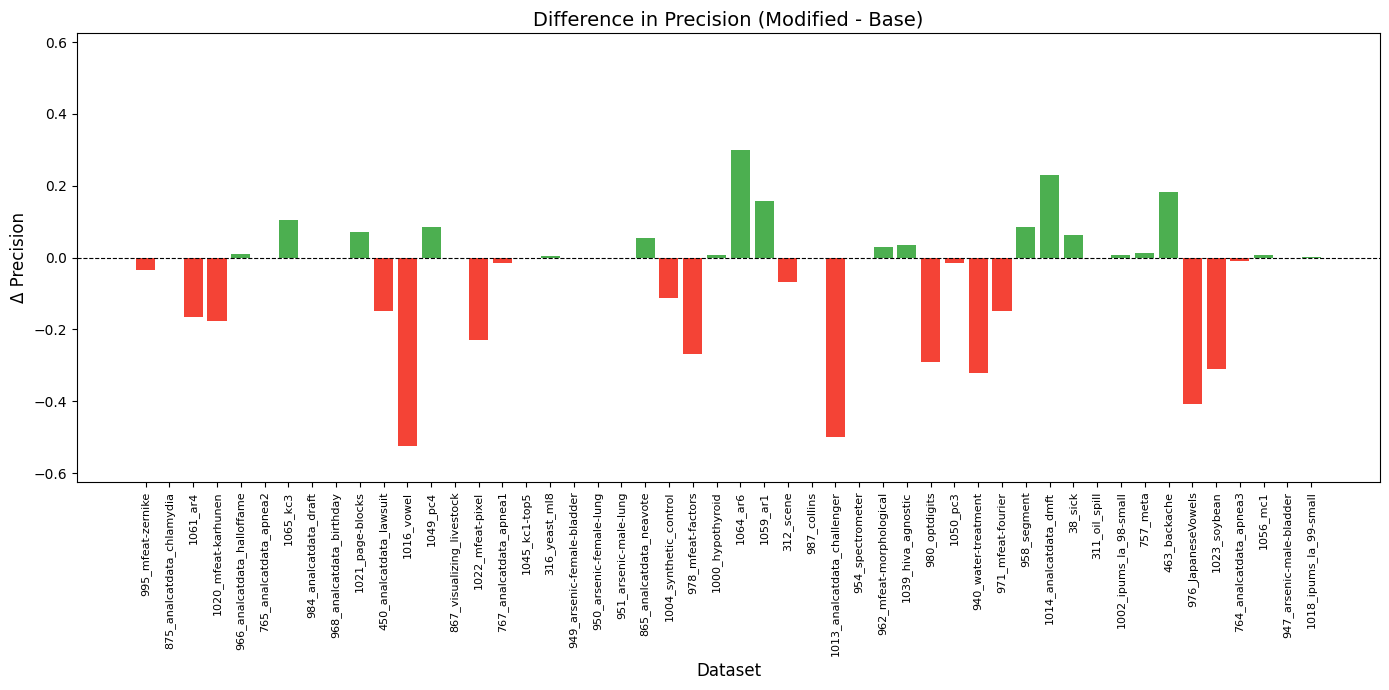
\includegraphics[width=.47\textwidth]{results/comparisons/precision_comparison.png}
            }%
            }
            \centerline{%
            \subfloat[Recall]{
                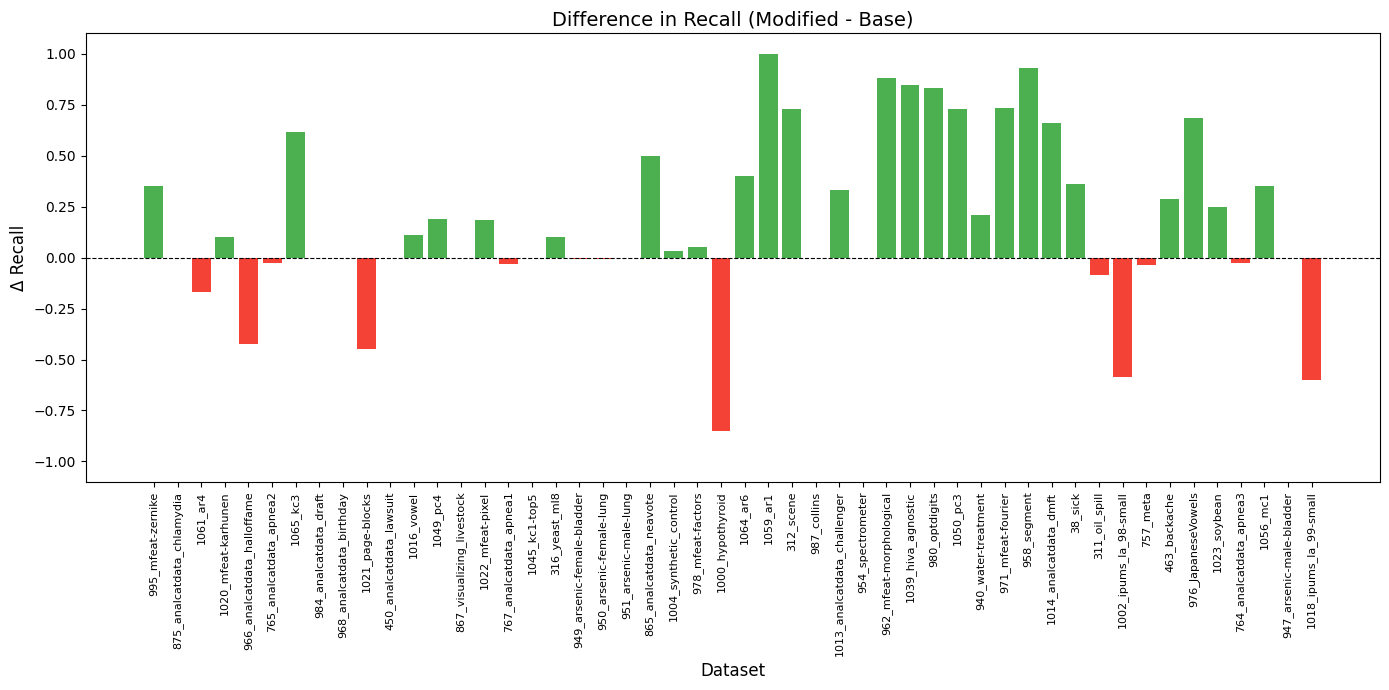
\includegraphics[width=.37\textwidth]{results/comparisons/recall_comparison.png}
            }%
            \subfloat[F1-Score]{
                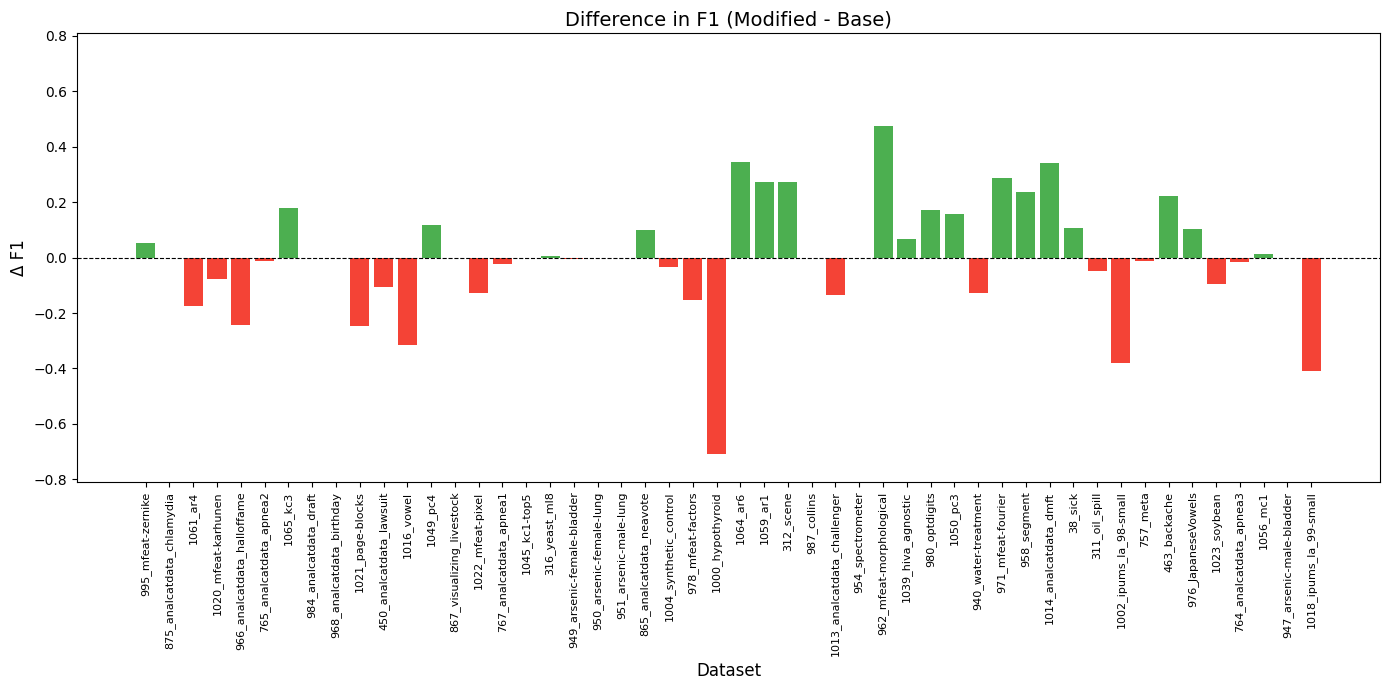
\includegraphics[width=.37\textwidth]{results/comparisons/f1_comparison.png}
            }%
            \subfloat[ROC]{
                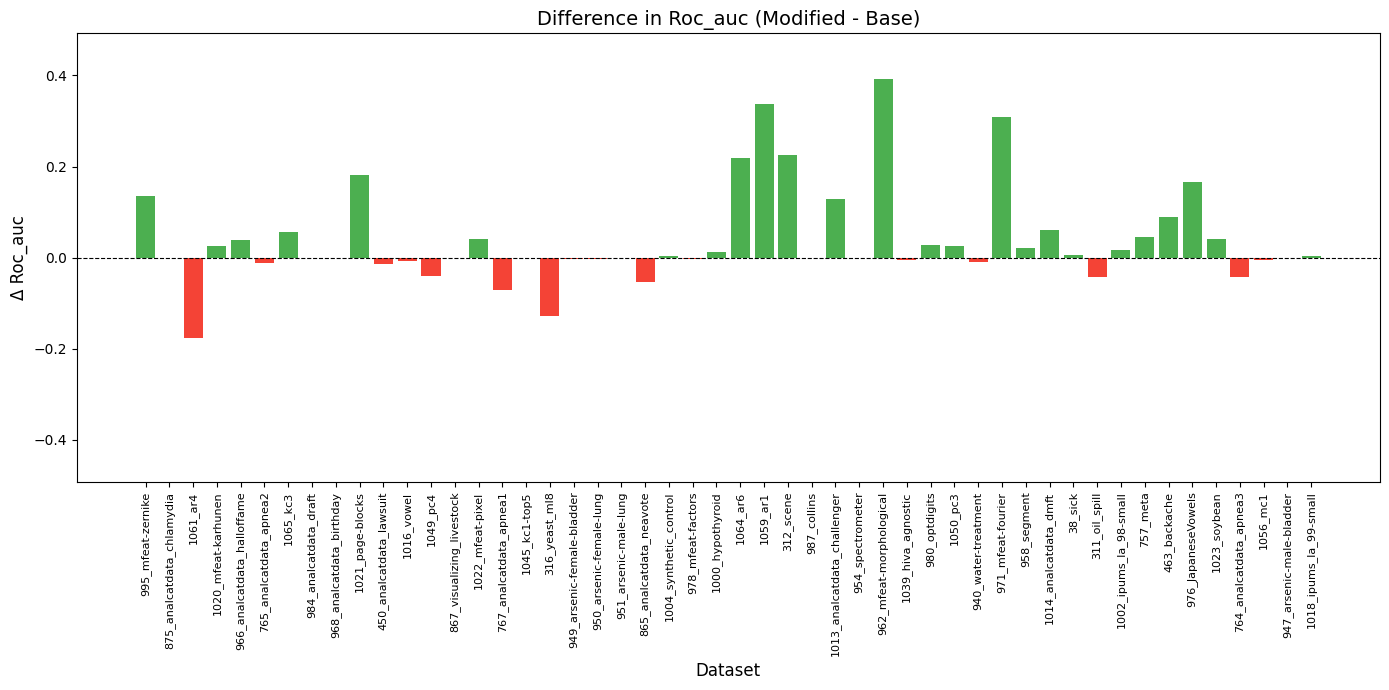
\includegraphics[width=.37\textwidth]{results/comparisons/roc_auc_comparison.png}
            }%% 
            }
    \end{figure}
\end{frame}

\begin{frame}{Empirical Study - Improvement Summary}
    \begin{figure}\centering
    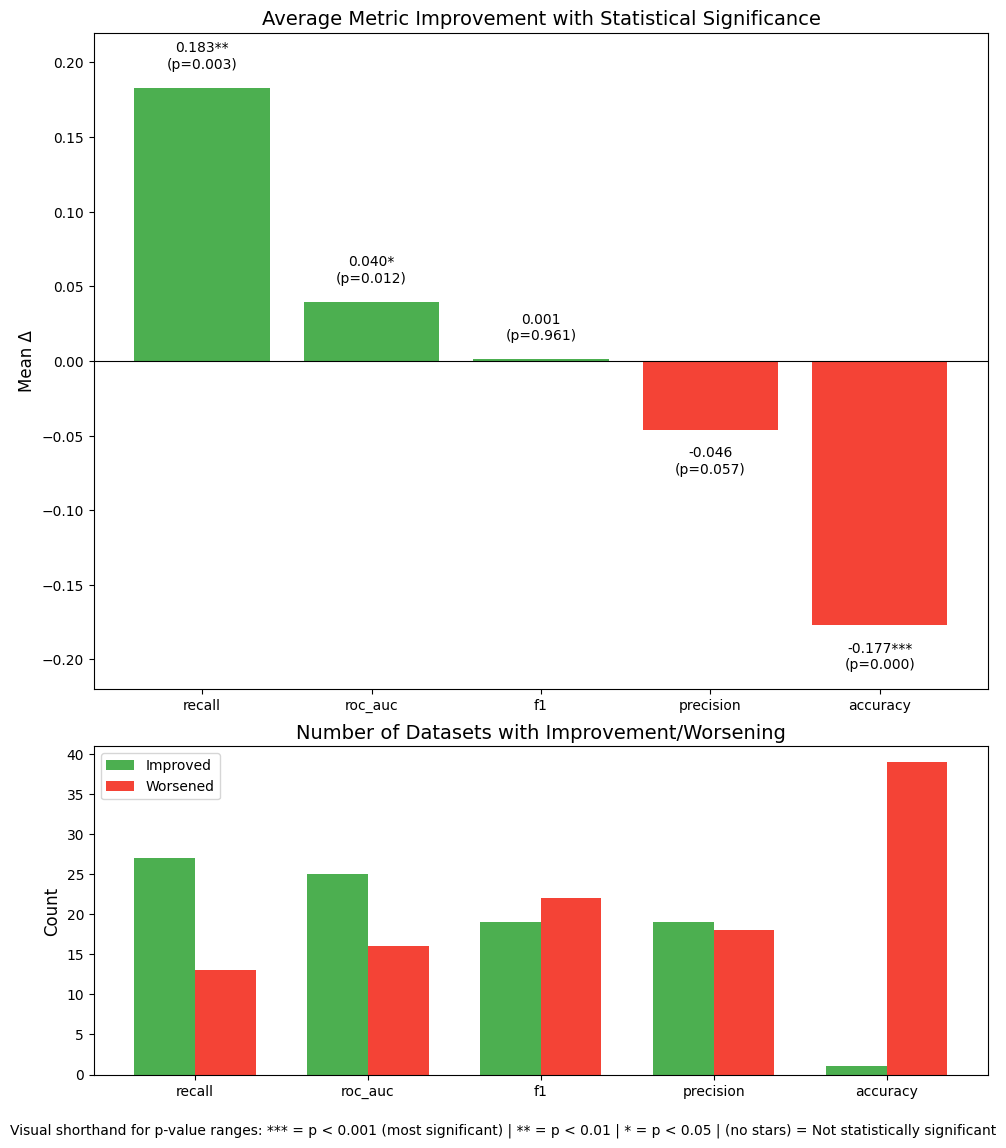
\includegraphics[width=.65\textwidth]{results/comparisons/improvement_summary.png}
    \end{figure}
\end{frame}

\begin{frame}{Conclusions and Future Work}
    \textbf{Key Findings:}
    \begin{itemize}
        \item {Modified CART Improves Minority-Class Performance:}
              \begin{itemize}
                  \item +4\% ROC-AUC
                  \item +18.3\% Recall
              \end{itemize}
        \item {Trade-offs Exist:}
              \begin{itemize}
                  \item Accuracy decreased 17.7\%
                  \item Gains were dataset-dependent
              \end{itemize}
    \end{itemize}
    \pause
    \textbf{Limitations:}
    \begin{itemize}
        \item Manual tuning of class weights required for each dataset.
        \item Noisy minority-class samples degrade performance.
    \end{itemize}
    \pause
    \textbf{Future Work:}
    \begin{itemize}
        \item Automate weight tuning via grid search.
    \end{itemize}
\end{frame}

\begin{frame}{References}    
    \begin{itemize}
        \item \textbf{CART Implementation (Base Code Inspiration):}
              \url{https://github.com/zziz/cart}

        \item \textbf{Original CART Algorithm:}
              Breiman, L., Friedman, J., Stone, C. J., \& Olshen, R. (1984).
              \textit{Classification and Regression Trees}. Chapman \& Hall/CRC.

        \item \textbf{Evaluation Metrics \& Tools:} 
            Hunter, J. D. (2007). \textit{Matplotlib: A 2D Graphics Environment}. IEEE.

    \end{itemize}
\end{frame}
\end{document}

